\section{\texttt{gWidgets}}

%----------------------------------------------------------------------

\subsection*{Descrição}

\begin{frame}

  \texttt{gWidgets} fornece um kit de ferramentas para construir
  interfaces gráficas interativas.

  \vspace{\baselineskip}

  Verzani, J., Lawrence, M. (2012). \emph{Programming Graphical User
    Interfaces in R}, CRC Press.

  \begin{itemize}
  \item Autor: John Verzani
  \item Lançamento: 29-Sep-2006
  \item Versão: 0.0-54
  \item URL: \url{http://cran.r-project.org/web/packages/gWidgets/index.html}
  \end{itemize}

\end{frame}

\begin{frame}

  \begin{itemize}
  \item Alguns pacotes baseados em toolkits suportadas:
    \begin{itemize}
    \item tcl/tk:
      \href{http://cran.r-project.org/web/packages/gWidgetstcltk/index.html}{\texttt{gWidgetstcltk}},
      \href{http://cran.r-project.org/web/packages/Rcmdr/index.html}{\texttt{Rcmdr}},
      \href{http://cran.r-project.org/web/packages/TeachingDemos/index.html}{\texttt{TeachingDemos}},
      \href{http://cran.r-project.org/web/packages/MetSizeR/index.html}{\texttt{MetSizeR}},
      \href{http://cran.r-project.org/web/packages/MergeGUI/index.html}{\texttt{MergeGUI}},
      \href{http://cran.r-project.org/web/packages/GrapheR/index.html}{\texttt{GrapheR}},
      \href{http://cran.r-project.org/web/packages/BiplotGUI/index.html}{\texttt{BiplotGUI}},
      \href{http://cran.r-project.org/web/packages/TestScorer/index.html}{\texttt{TestScorer}}
      e muitos outros.
    \item gtk:
      \href{http://cran.r-project.org/web/packages/gWidgetsRGtk2/index.html}{\texttt{gWidgetsRGtk2}},
      \href{http://cran.r-project.org/web/packages/playwith/index.html}{\texttt{playwith}},
      \href{http://cran.r-project.org/web/packages/MissingDataGUI/index.html}{\texttt{MissingDataGUI}},
      \href{http://cran.r-project.org/web/packages/GroupSeq/index.html}{\texttt{GroupSeq}},
      \href{http://cran.r-project.org/web/packages/AtelieR/index.html}{\texttt{AtelieR}},
      \href{http://cran.r-project.org/web/packages/vmsbase/index.html}{\texttt{vmsbase}},
      \href{http://cran.r-project.org/web/packages/reshapeGUI/index.html}{\texttt{reshapeGUI}},
      \href{http://cran.r-project.org/web/packages/R2STATS/index.html}{\texttt{R2STATS}}
      e muitos outros.
  \end{itemize}
\end{itemize}

\end{frame}

%----------------------------------------------------------------------

\subsection*{Como usar}

\begin{frame}
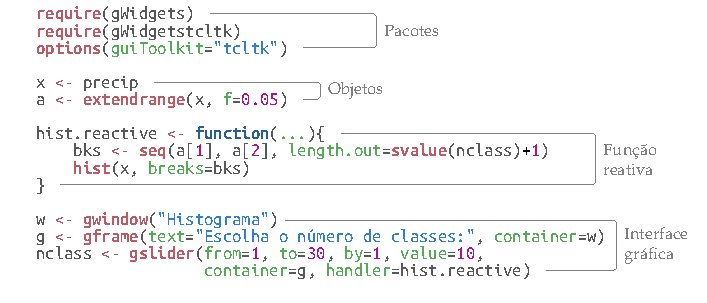
\includegraphics[scale=1]{./tikz/hist_slider_gWidgets-1.pdf}
\end{frame}

\begin{frame}
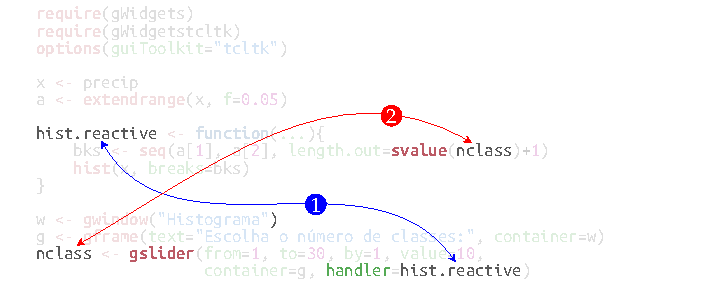
\includegraphics[scale=1]{./tikz/hist_slider_gWidgets-2.pdf}
\end{frame}

%----------------------------------------------------------------------

\subsection*{Exemplos}

\begin{frame}
 Praticando:
  \begin{enumerate}
  \item
    \href{run:./R/gWidgets/gWidgets.R}{R Script gWidgets}
  \item 
	\href{run:gWidgets.html}{Galeria gWidgets IGUIR}
  \end{enumerate}

  \vspace{0.5cm}
  Algumas aplicações com o gWidgets:
  \begin{itemize}
  \item \href{http://cran.r-project.org/web/packages/gWidgets/vignettes/}{Galeria
      do autor},
  \item \href{https://github.com/jverzani/ProgGUIinR}{ProGUIinR Package},
  \item \href{http://www.r-bloggers.com/?s=gWidgets}{Busca no R
      Bloggers}
  \end{itemize}
\end{frame}

